% Created by tikzDevice version 0.12.6 on 2026-07-06 23:55:44
% !TEX encoding = UTF-8 Unicode
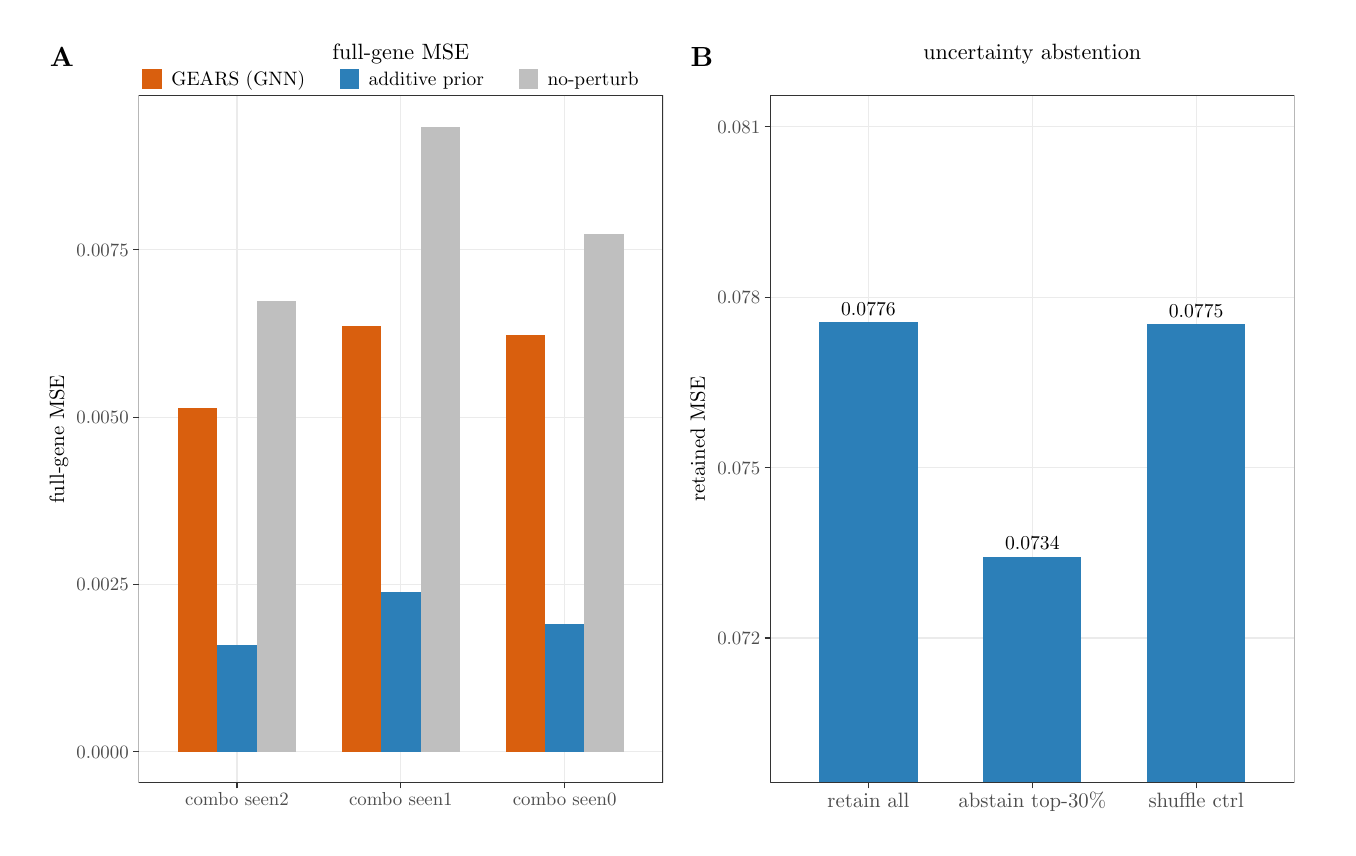
\begin{tikzpicture}[x=1pt,y=1pt]
\definecolor{fillColor}{RGB}{255,255,255}
\path[use as bounding box,fill=fillColor,fill opacity=0.00] (0,0) rectangle (469.75,289.08);
\begin{scope}
\path[clip] (  0.00,  0.00) rectangle (469.75,289.08);
\definecolor{drawColor}{RGB}{255,255,255}
\definecolor{fillColor}{RGB}{255,255,255}

\path[draw=drawColor,line width= 0.4pt,line join=round,line cap=round,fill=fillColor] ( -0.00,  0.00) rectangle (469.76,289.08);
\end{scope}
\begin{scope}
\path[clip] (  4.00,  3.00) rectangle (235.58,286.08);
\definecolor{drawColor}{RGB}{255,255,255}
\definecolor{fillColor}{RGB}{255,255,255}

\path[draw=drawColor,line width= 0.4pt,line join=round,line cap=round,fill=fillColor] (  4.00,  3.00) rectangle (235.58,286.08);
\end{scope}
\begin{scope}
\path[clip] (235.58,  3.00) rectangle (463.76,286.08);
\definecolor{drawColor}{RGB}{255,255,255}
\definecolor{fillColor}{RGB}{255,255,255}

\path[draw=drawColor,line width= 0.4pt,line join=round,line cap=round,fill=fillColor] (235.58,  3.00) rectangle (463.76,286.08);
\end{scope}
\begin{scope}
\path[clip] ( 40.11, 16.22) rectangle (229.58,264.52);
\definecolor{fillColor}{RGB}{255,255,255}

\path[fill=fillColor] ( 40.11, 16.22) rectangle (229.58,264.52);
\definecolor{drawColor}{gray}{0.92}

\path[draw=drawColor,line width= 0.4pt,line join=round] ( 40.11, 27.51) --
	(229.58, 27.51);

\path[draw=drawColor,line width= 0.4pt,line join=round] ( 40.11, 87.93) --
	(229.58, 87.93);

\path[draw=drawColor,line width= 0.4pt,line join=round] ( 40.11,148.34) --
	(229.58,148.34);

\path[draw=drawColor,line width= 0.4pt,line join=round] ( 40.11,208.76) --
	(229.58,208.76);

\path[draw=drawColor,line width= 0.4pt,line join=round] ( 75.63, 16.22) --
	( 75.63,264.52);

\path[draw=drawColor,line width= 0.4pt,line join=round] (134.84, 16.22) --
	(134.84,264.52);

\path[draw=drawColor,line width= 0.4pt,line join=round] (194.05, 16.22) --
	(194.05,264.52);
\definecolor{fillColor}{RGB}{217,95,14}

\path[fill=fillColor] ( 54.32, 27.51) rectangle ( 68.53,151.73);
\definecolor{fillColor}{RGB}{44,127,184}

\path[fill=fillColor] ( 68.53, 27.51) rectangle ( 82.74, 65.93);
\definecolor{fillColor}{gray}{0.75}

\path[fill=fillColor] ( 82.74, 27.51) rectangle ( 96.95,190.39);
\definecolor{fillColor}{RGB}{217,95,14}

\path[fill=fillColor] (113.53, 27.51) rectangle (127.74,181.21);
\definecolor{fillColor}{RGB}{44,127,184}

\path[fill=fillColor] (127.74, 27.51) rectangle (141.95, 85.27);
\definecolor{fillColor}{gray}{0.75}

\path[fill=fillColor] (141.95, 27.51) rectangle (156.16,253.23);
\definecolor{fillColor}{RGB}{217,95,14}

\path[fill=fillColor] (172.74, 27.51) rectangle (186.95,178.07);
\definecolor{fillColor}{RGB}{44,127,184}

\path[fill=fillColor] (186.95, 27.51) rectangle (201.16, 73.43);
\definecolor{fillColor}{gray}{0.75}

\path[fill=fillColor] (201.16, 27.51) rectangle (215.37,214.56);
\definecolor{drawColor}{gray}{0.20}

\path[draw=drawColor,line width= 0.4pt,line join=round,line cap=round] ( 40.11, 16.22) rectangle (229.58,264.52);
\end{scope}
\begin{scope}
\path[clip] (  0.00,  0.00) rectangle (469.75,289.08);
\definecolor{drawColor}{gray}{0.30}

\node[text=drawColor,anchor=base east,inner sep=0pt, outer sep=0pt, scale=  0.68] at ( 36.51, 25.17) {0.0000};

\node[text=drawColor,anchor=base east,inner sep=0pt, outer sep=0pt, scale=  0.68] at ( 36.51, 85.59) {0.0025};

\node[text=drawColor,anchor=base east,inner sep=0pt, outer sep=0pt, scale=  0.68] at ( 36.51,146.00) {0.0050};

\node[text=drawColor,anchor=base east,inner sep=0pt, outer sep=0pt, scale=  0.68] at ( 36.51,206.42) {0.0075};
\end{scope}
\begin{scope}
\path[clip] (  0.00,  0.00) rectangle (469.75,289.08);
\definecolor{drawColor}{gray}{0.20}

\path[draw=drawColor,line width= 0.4pt,line join=round] ( 38.11, 27.51) --
	( 40.11, 27.51);

\path[draw=drawColor,line width= 0.4pt,line join=round] ( 38.11, 87.93) --
	( 40.11, 87.93);

\path[draw=drawColor,line width= 0.4pt,line join=round] ( 38.11,148.34) --
	( 40.11,148.34);

\path[draw=drawColor,line width= 0.4pt,line join=round] ( 38.11,208.76) --
	( 40.11,208.76);
\end{scope}
\begin{scope}
\path[clip] (  0.00,  0.00) rectangle (469.75,289.08);
\definecolor{drawColor}{gray}{0.20}

\path[draw=drawColor,line width= 0.4pt,line join=round] ( 75.63, 14.22) --
	( 75.63, 16.22);

\path[draw=drawColor,line width= 0.4pt,line join=round] (134.84, 14.22) --
	(134.84, 16.22);

\path[draw=drawColor,line width= 0.4pt,line join=round] (194.05, 14.22) --
	(194.05, 16.22);
\end{scope}
\begin{scope}
\path[clip] (  0.00,  0.00) rectangle (469.75,289.08);
\definecolor{drawColor}{gray}{0.30}

\node[text=drawColor,anchor=base,inner sep=0pt, outer sep=0pt, scale=  0.68] at ( 75.63,  7.94) {combo seen2};

\node[text=drawColor,anchor=base,inner sep=0pt, outer sep=0pt, scale=  0.68] at (134.84,  7.94) {combo seen1};

\node[text=drawColor,anchor=base,inner sep=0pt, outer sep=0pt, scale=  0.68] at (194.05,  7.94) {combo seen0};
\end{scope}
\begin{scope}
\path[clip] (  0.00,  0.00) rectangle (469.75,289.08);
\definecolor{drawColor}{RGB}{0,0,0}

\node[text=drawColor,rotate= 90.00,anchor=base,inner sep=0pt, outer sep=0pt, scale=  0.75] at ( 13.17,140.37) {full-gene MSE};
\end{scope}
\begin{scope}
\path[clip] (  0.00,  0.00) rectangle (469.75,289.08);
\definecolor{fillColor}{RGB}{255,255,255}

\path[fill=fillColor] ( 39.92,266.52) rectangle (229.76,274.52);
\end{scope}
\begin{scope}
\path[clip] (  0.00,  0.00) rectangle (469.75,289.08);
\definecolor{fillColor}{RGB}{255,255,255}

\path[fill=fillColor] ( 40.92,266.52) rectangle ( 48.92,274.52);
\definecolor{fillColor}{RGB}{217,95,14}

\path[fill=fillColor] ( 41.44,267.03) rectangle ( 48.41,274.00);
\end{scope}
\begin{scope}
\path[clip] (  0.00,  0.00) rectangle (469.75,289.08);
\definecolor{fillColor}{RGB}{255,255,255}

\path[fill=fillColor] (112.23,266.52) rectangle (120.23,274.52);
\definecolor{fillColor}{RGB}{44,127,184}

\path[fill=fillColor] (112.75,267.03) rectangle (119.71,274.00);
\end{scope}
\begin{scope}
\path[clip] (  0.00,  0.00) rectangle (469.75,289.08);
\definecolor{fillColor}{RGB}{255,255,255}

\path[fill=fillColor] (176.87,266.52) rectangle (184.87,274.52);
\definecolor{fillColor}{gray}{0.75}

\path[fill=fillColor] (177.39,267.03) rectangle (184.35,274.00);
\end{scope}
\begin{scope}
\path[clip] (  0.00,  0.00) rectangle (469.75,289.08);
\definecolor{drawColor}{RGB}{0,0,0}

\node[text=drawColor,anchor=base west,inner sep=0pt, outer sep=0pt, scale=  0.70] at ( 51.92,268.10) {GEARS (GNN)};
\end{scope}
\begin{scope}
\path[clip] (  0.00,  0.00) rectangle (469.75,289.08);
\definecolor{drawColor}{RGB}{0,0,0}

\node[text=drawColor,anchor=base west,inner sep=0pt, outer sep=0pt, scale=  0.70] at (123.23,268.10) {additive prior};
\end{scope}
\begin{scope}
\path[clip] (  0.00,  0.00) rectangle (469.75,289.08);
\definecolor{drawColor}{RGB}{0,0,0}

\node[text=drawColor,anchor=base west,inner sep=0pt, outer sep=0pt, scale=  0.70] at (187.87,268.10) {no-perturb};
\end{scope}
\begin{scope}
\path[clip] (  0.00,  0.00) rectangle (469.75,289.08);
\definecolor{drawColor}{RGB}{0,0,0}

\node[text=drawColor,anchor=base,inner sep=0pt, outer sep=0pt, scale=  0.80] at (134.84,277.57) {full-gene MSE};
\end{scope}
\begin{scope}
\path[clip] (  0.00,  0.00) rectangle (469.75,289.08);
\definecolor{drawColor}{RGB}{0,0,0}

\node[text=drawColor,anchor=base,inner sep=0pt, outer sep=0pt, scale=  1.00] at ( 12.35,275.21) {\bfseries A};
\end{scope}
\begin{scope}
\path[clip] (268.29, 16.22) rectangle (457.76,264.52);
\definecolor{fillColor}{RGB}{255,255,255}

\path[fill=fillColor] (268.29, 16.22) rectangle (457.76,264.52);
\definecolor{drawColor}{gray}{0.92}

\path[draw=drawColor,line width= 0.4pt,line join=round] (268.29, 68.55) --
	(457.76, 68.55);

\path[draw=drawColor,line width= 0.4pt,line join=round] (268.29,130.11) --
	(457.76,130.11);

\path[draw=drawColor,line width= 0.4pt,line join=round] (268.29,191.67) --
	(457.76,191.67);

\path[draw=drawColor,line width= 0.4pt,line join=round] (268.29,253.23) --
	(457.76,253.23);

\path[draw=drawColor,line width= 0.4pt,line join=round] (303.81, 16.22) --
	(303.81,264.52);

\path[draw=drawColor,line width= 0.4pt,line join=round] (363.02, 16.22) --
	(363.02,264.52);

\path[draw=drawColor,line width= 0.4pt,line join=round] (422.23, 16.22) --
	(422.23,264.52);
\definecolor{fillColor}{RGB}{44,127,184}

\path[fill=fillColor] (286.05,-1408.89) rectangle (321.57,182.64);

\path[fill=fillColor] (345.26,-1408.89) rectangle (380.78, 97.89);

\path[fill=fillColor] (404.47,-1408.89) rectangle (439.99,182.02);
\definecolor{drawColor}{RGB}{0,0,0}

\node[text=drawColor,anchor=base,inner sep=0pt, outer sep=0pt, scale=  0.71] at (303.81,185.09) {0.0776};

\node[text=drawColor,anchor=base,inner sep=0pt, outer sep=0pt, scale=  0.71] at (363.02,100.34) {0.0734};

\node[text=drawColor,anchor=base,inner sep=0pt, outer sep=0pt, scale=  0.71] at (422.23,184.47) {0.0775};
\definecolor{drawColor}{gray}{0.20}

\path[draw=drawColor,line width= 0.4pt,line join=round,line cap=round] (268.29, 16.22) rectangle (457.76,264.52);
\end{scope}
\begin{scope}
\path[clip] (  0.00,  0.00) rectangle (469.75,289.08);
\definecolor{drawColor}{gray}{0.30}

\node[text=drawColor,anchor=base east,inner sep=0pt, outer sep=0pt, scale=  0.68] at (264.69, 66.21) {0.072};

\node[text=drawColor,anchor=base east,inner sep=0pt, outer sep=0pt, scale=  0.68] at (264.69,127.77) {0.075};

\node[text=drawColor,anchor=base east,inner sep=0pt, outer sep=0pt, scale=  0.68] at (264.69,189.33) {0.078};

\node[text=drawColor,anchor=base east,inner sep=0pt, outer sep=0pt, scale=  0.68] at (264.69,250.89) {0.081};
\end{scope}
\begin{scope}
\path[clip] (  0.00,  0.00) rectangle (469.75,289.08);
\definecolor{drawColor}{gray}{0.20}

\path[draw=drawColor,line width= 0.4pt,line join=round] (266.29, 68.55) --
	(268.29, 68.55);

\path[draw=drawColor,line width= 0.4pt,line join=round] (266.29,130.11) --
	(268.29,130.11);

\path[draw=drawColor,line width= 0.4pt,line join=round] (266.29,191.67) --
	(268.29,191.67);

\path[draw=drawColor,line width= 0.4pt,line join=round] (266.29,253.23) --
	(268.29,253.23);
\end{scope}
\begin{scope}
\path[clip] (  0.00,  0.00) rectangle (469.75,289.08);
\definecolor{drawColor}{gray}{0.20}

\path[draw=drawColor,line width= 0.4pt,line join=round] (303.81, 14.22) --
	(303.81, 16.22);

\path[draw=drawColor,line width= 0.4pt,line join=round] (363.02, 14.22) --
	(363.02, 16.22);

\path[draw=drawColor,line width= 0.4pt,line join=round] (422.23, 14.22) --
	(422.23, 16.22);
\end{scope}
\begin{scope}
\path[clip] (  0.00,  0.00) rectangle (469.75,289.08);
\definecolor{drawColor}{gray}{0.30}

\node[text=drawColor,anchor=base,inner sep=0pt, outer sep=0pt, scale=  0.75] at (303.81,  7.46) {retain all};

\node[text=drawColor,anchor=base,inner sep=0pt, outer sep=0pt, scale=  0.75] at (363.02,  7.46) {abstain top-30\%};

\node[text=drawColor,anchor=base,inner sep=0pt, outer sep=0pt, scale=  0.75] at (422.23,  7.46) {shuffle ctrl};
\end{scope}
\begin{scope}
\path[clip] (  0.00,  0.00) rectangle (469.75,289.08);
\definecolor{drawColor}{RGB}{0,0,0}

\node[text=drawColor,rotate= 90.00,anchor=base,inner sep=0pt, outer sep=0pt, scale=  0.75] at (244.74,140.37) {retained MSE};
\end{scope}
\begin{scope}
\path[clip] (  0.00,  0.00) rectangle (469.75,289.08);
\definecolor{drawColor}{RGB}{0,0,0}

\node[text=drawColor,anchor=base,inner sep=0pt, outer sep=0pt, scale=  0.80] at (363.02,277.57) {uncertainty abstention};
\end{scope}
\begin{scope}
\path[clip] (  0.00,  0.00) rectangle (469.75,289.08);
\definecolor{drawColor}{RGB}{0,0,0}

\node[text=drawColor,anchor=base,inner sep=0pt, outer sep=0pt, scale=  1.00] at (243.67,275.21) {\bfseries B};
\end{scope}
\end{tikzpicture}
